%!TEX root = ./main.tex

% content goes here    
    \section{Recap}
	\begin{frame}
		\frametitle{Recap}
		% \framesubtitle{}
		\begin{columns}[c]
    		\column{.5\textwidth} 
        		\begin{itemize}
					\item Collaborate
                    \item Version Control
                    \item Open Source
          		\end{itemize}
          	\column{.5\textwidth}
            	\centering
				
\includegraphics[width=.7\linewidth,]{res/git}

				\vspace{1cm} % blank lines around this are needed

				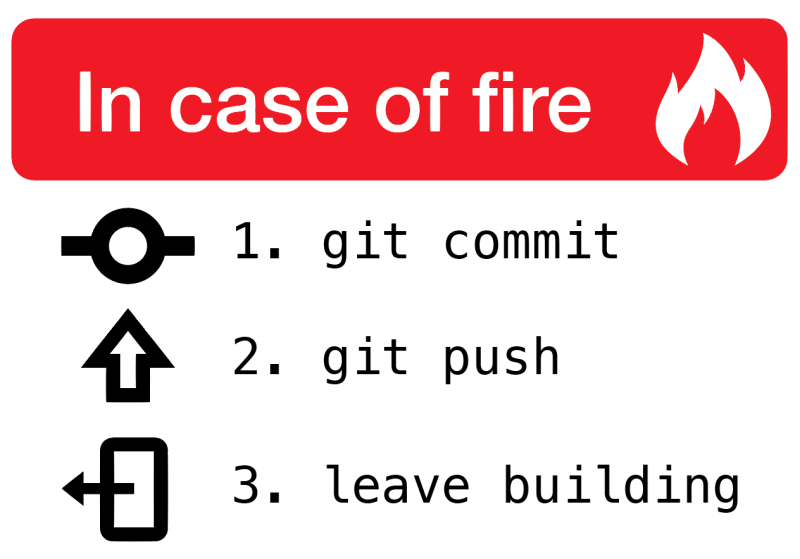
\includegraphics[width=.7\linewidth]{res/fire}
        \end{columns}
	\end{frame}
	
	\section{Account}
	\begin{frame}
		\frametitle{Create a git account I}
		\begin{center}
		\begin{tabular}{l | l}
			Acount & \link{https://github.com/}{GitHub}\\
			Stundent pack & \link{https://education.github.com/pack}{Student developer pack}
		
		\end{tabular}
		\end{center}
	\end{frame}
    
    \begin{frame} 
		\frametitle{Create a git account II}
		\begin{itemize}
			\item Gebruik studentenmail: voornaam.achternaam@student.uantwerpen.be
			\item Gebruik herkenbare naam
		\end{itemize}

	
		\begin{itemize}
			\item \textbf{Student pack geeft mogelijkheid tot private repositories!}
		\end{itemize}
		
	\end{frame}
	
	\section{SSH key}
	\begin{frame}
		\frametitle{SSH key}
		Geen wachtwoord en gebruikersnaam meer in te vullen!
		
		\begin{enumerate}
		\item \link{https://help.github.com/en/github/authenticating-to-github/generating-a-new-ssh-key-and-adding-it-to-the-ssh-agent}{Generate SSH key}
		
		\item \link{https://help.github.com/en/github/authenticating-to-github/adding-a-new-ssh-key-to-your-github-account}{Add key to github account}
		\end{enumerate}
		
	\end{frame}
	
	\begin{frame}
	\frametitle{Git clone}
	\begin{center}
		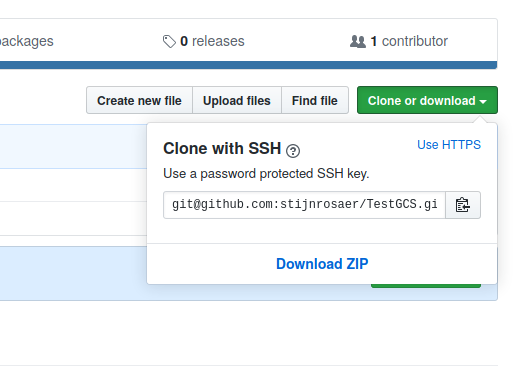
\includegraphics[scale=0.5]{res/sshGitRepo.png}
	\end{center}
	
	\end{frame}
	
	
	\section{Git in terminal}
	\begin{frame}
	\frametitle{Commands}
		\begin{itemize}
			\item git clone
			\item git pull
			\item \textbf{git status}
			\item git commit -m ""
			\item git push
		\end{itemize}
	\end{frame}
	
	\begin{frame}
	\frametitle{Cheat sheet}
	\link{https://education.github.com/git-cheat-sheet-education.pdf}{Cheat sheet}
	\end{frame}
	
	\section{Oefening}
	\begin{frame}
	\frametitle{Oefening I}
	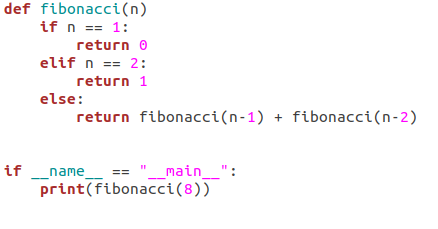
\includegraphics[scale=0.5]{res/fib.png}
	\end{frame}
	
	\begin{frame}
	\frametitle{Oefening II}
	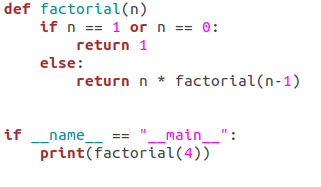
\includegraphics[scale=0.5]{res/fac.png}
	\end{frame}
	
	\section{git status}
	\begin{frame}
	\frametitle{Git status}
		\begin{center}
			{\Huge {\textbf{GIT STATUS?}}}
		\end{center}	
	\end{frame}

	
	
	
	
	
	

	% end of content
